\documentclass[10pt,a4paper,oneside]{article}

\usepackage{listings}
\usepackage{color}

\definecolor{codegreen}{rgb}{0,0.6,0}
\definecolor{codegray}{rgb}{0.5,0.5,0.5}
\definecolor{codepurple}{rgb}{0.58,0,0.82}
\definecolor{backcolour}{rgb}{0.95,0.95,0.92}
 
\lstdefinestyle{mystyle}{
    backgroundcolor=\color{backcolour},   
    commentstyle=\color{codegreen},
    keywordstyle=\color{magenta},
    numberstyle=\tiny\color{codegray},
    stringstyle=\color{codepurple},
    basicstyle=\footnotesize,
    breakatwhitespace=false,         
    breaklines=true,                 
    captionpos=b,                    
    keepspaces=true,                 
    numbers=left,                    
    numbersep=5pt,                  
    showspaces=false,                
    showstringspaces=false,
    showtabs=false,                  
    tabsize=2
}
 
\lstset{style=mystyle}


\usepackage[utf8]{inputenc}
\usepackage{verbatim}
\usepackage[T1]{fontenc}
\usepackage{amsmath}
\usepackage{amsfonts}
\usepackage{amssymb}
\usepackage{graphicx}
\usepackage[left=2cm,right=2cm,top=2cm,bottom=2cm]{geometry}
\usepackage{multicol}
\usepackage{amsthm}
\author{Baptiste Chanus}

\title{Utilisation d'IA pour anticiper les pannes des architectures en nuage basées sur des micro-service et des conteneurs}

\begin{document}

\begin{center}

\vspace{0.8cm}

\begin{Large}
Utilisation d'IA pour anticiper les pannes des architectures en nuage basées sur des micro-service et des conteneurs
\end{Large}
\end{center}

\vspace{0.8cm}

\begin{figure}[h!]
\centering

\includegraphics[scale=0.5]{./images/PNG/scc-logo.png}
\end{figure}

\vspace{0.8cm}

Author: Chanus Baptiste\\
Coordinator: Aubertin Michael\\
Contact: maubertin@fr.scc.com\\

\vspace{0.8cm}

\begin{abstract}
Dans l’ensemble de l’industrie, de nombreux systèmes reposent sur la stabilité du cloud, du réseau, du datacenter et des composants logiciels. Ainsi, chaque application doit être disponible la plupart du temps. En outre, le modèle de gouvernance informatique incite les équipes informatiques à prendre des engagements forts en matière de responsabilité afin de remédier aux pannes le plus rapidement possible. Ce travail concerne un algorithme d’apprentissage dont le but est de donner un indice sur le moment où une indisponibilité va se produire. En coopération avec les systèmes de surveillance utilisés pour collecter les données sur la disponibilité des applications, comme les logiciels basés sur nagios, l’algorithme vise à traiter les données en rassemblant peu de techniques classiques différentes, telles que l’algorithme génétique de réseau neuronal. Cette méthode est cependant en quelque sorte basée sur des pensées empiriques et vise à deviner un échec avant qu'il ne se produise.
\end{abstract}

\vspace{1.2cm}

\begin{multicols}{2}
\section{Introduction}
Les applications contractées s'exécutent avec un délai maximal d'indisponibilité par jour. Ainsi, lorsqu'un incident se produit, une course contre la montre commence. Le problème doit être diagnostiqué et résolu le plus rapidement possible car il engage l'indicateur qualité qu'est le temps d'indisponibilité. Cet  indicateur de performance clés est un des plus importants KPI d’un accord de niveau de service contracté avec des services informatiques de classe industrielle. Nous essayons ici de trouver une solution qui pourrait aider à anticiper ces problèmes afin que le temps de résolution soit le plus court possible.
\\
Lorsque, en 2017, nous avons essayé de trouver une solution au problème, nous avons décidé d'utiliser les fichiers journaux des systèmes de surveillance basés sur Nagios auxquels nous avions accès. Nous pensions que nous pouvions établir un processus d’apprentissage en utilisant uniquement les données de disponibilité de nagios (décrites dans la partie suivante) pour prévoir toute défaillance de l’application. Toute la solution initiale est expliquée en détail tout au long de la première partie, mais repose sur l'hypothèse selon laquelle les modifications apportées à la structure de l'application sont rares, ce qui était une hypothèse cohérente à cette époque.
\\ 
Cependant, les technologies ont évolué et les applications peuvent avoir de petites modifications dans leur structure régulièrement. Cela rend toute forme d'apprentissage assez difficile, car l'entrainement de l'IA est réalisée avec une structure spécifique de l'application. Ce changement d’architecture est généralement celui attendu d’un nouveau type d’infrastructure, comme par exemple les applications conteneurisées orchestrées. C’est pourquoi, dans une deuxième partie, nous nous concentrerons sur la manière de cibler des hôtes spécifiques, ceux qui ont le plus d’influence sur l’état de l’application, afin de pouvoir appliquer notre méthode d’apprentissage précédente à un sous-ensemble de tous les hôtes de l’application qui ne change pas trop. Enfin, nous essaierons également de regrouper certains hôtes de telle sorte que certains puissent être ajoutés ou supprimés du système d'information tout en étant pris en compte et que l'apprentissage ne soit pas affecté par les changements de structure.
\end{multicols}


\begin{multicols}{2}
\section{Méthode basée sur les disponibilités}
Cette première méthode utilise les données de disponibilité nagios, ce qui signifie que nous n’avons accès, pour chaque hôte et service de l’application, qu’au score d'état de disponibilité compris entre 0 et 3 (0: OK, 1: Avertissement, 2: Critique, 3: Inconnu). Nous allons utiliser les données historiques d'anciens journaux pour entrainer un algorithme d'apprentissage automatique combinant deux techniques d'apprentissage. La première s'appuye sur des réseaux de neurones et ensuite un principe d'algorithme génétique que nous utiliserons ensuite sur les données réelles pour prédire la panne de l'application qui en résultera. éventuellement se produire. Cependant, comme expliqué dans l'introduction, cette méthode pose de sérieux problèmes de rigidité car la formation est faite sur la structure d'une application spécifique. Nous allons discuter de cette limite en tant que conclusion de cette méthode.
\subsection{Modelisation des applications}
La modèlisation d'application choisie est un arbre de dépendances. L'application est la racine de l'arborescence, les nœuds internes sont les hôtes et les feuilles sont les services. À chaque nœud, une relation est associée à ses enfants. Cette porte logique indique si tous sont requis pour la disponibilité de ce nœud ou si certains peuvent être en panne sans rendre ce nœud indisponible. Ces relations ne sont que des relations connues, ce qui signifie qu’elles sont explicites et évidentes lors de la conception de l’application. Nous pouvons avoir des relations qui sont impliquées par l'interaction des nœuds internes qui se produit dans un système de la vie réelle sans que nous en soyons conscients, mais elles ne sont pas évidentes lors du processus de création de l'application. (voir ci-dessous Figure~\ref{exampletree})
\end{multicols}

\vspace{0.8cm}

\begin{figure}
\centering
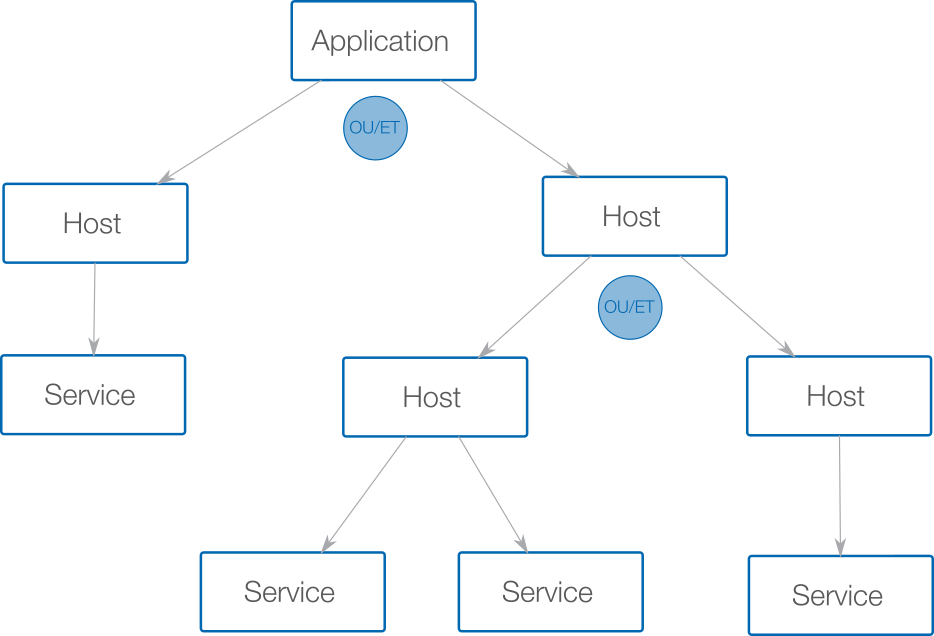
\includegraphics[scale=0.5]{./images/PNG/abrerelation.png}
\caption{Exemple d'arbre}
\label{exampletree}
\end{figure}

\vspace{0.8cm}

\begin{multicols}{2}
Nous définissons également une image comme étant l’état de l’ensemble de l’application, c’est-à-dire l’état de tous ses composants (hôtes et services) à un moment donné. Ceci est représenté sous la forme d'un tableau contenant 4 lignes, une pour chaque état (0-3) et autant de colonnes que d'hôtes et de services. L'état d'un hôte ou d'un service est donné par un booléen dans le tableau (true dans la ligne correspondant à l'état correspondant et false partout ailleurs), illustré à la figure~\ref{tab}

\end{multicols}

\vspace{0.8cm}

\begin{figure}[!h]
\centering
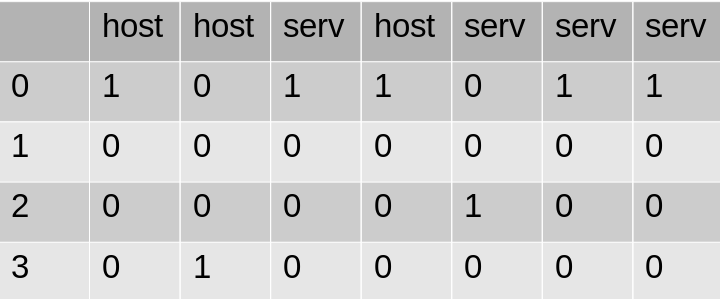
\includegraphics[scale=0.5]{./images/image.png}
\caption{Matrice d'état}
\label{tab}
\end{figure}

\vspace{0.8cm}


\begin{multicols}{2}
\subsection{Traitement des données}
Nous allons utiliser l'apprentissage automatique supervisé. Par conséquent, nous devons étiqueter les données historiques que nous utiliserons pour former notre réseau de neurones. Le réseau de neurones devra deviner le nombre d'époques restant jusqu'à la prochaine panne. Nous devons donc extraire du journal toutes les époques où l'application était inégalable. Ceci peut être réalisé avec une requête à la base de données dans laquelle sont stockées toutes les dates du début et de la fin d'une panne, puis en modulant les images dont l'époque se situe entre le début et la fin.
  De plus, nous devons associer à chaque image le temps restant avant la prochaine panne. Cela peut être fait facilement en utilisant ce que nous avions calculé auparavant.
\\Nous calculons maintenant une moyenne de toutes les images précédant immédiatement une panne. À ce stade, nous avons fait une hypothèse. Nous avons supposé que suffisamment d'informations avaient été collectées pour alimenter le réseau de neurones et qu'une estimation raisonnablement précise serait stockée dans la comparaison entre une image et la moyenne calculée. Nous allons appeler cette image moyenne la référence.
\\La comparaison entre une image et la référence se fait en utilisant un simple calcul de distance entre coordonnées, c’est-à-dire en notant $a_{i}$ les coordonnées de l’image et $r_{i}$ celles de la référence que nous utilisons, pour un $k\in\mathbb{N}$ donné, la formule suivante:

\vspace{0.8cm}

\begin{Large}
\[ d(a, r) = \sqrt[k]{\sum \mid{a_i - r_i}\mid^{k}} \]
\end{Large}

\vspace{0.8cm}

\subsection{Réseaux de Neurones}
Le premier apprentissage de l'algorithme se fait via des réseaux de neurones. Nous allons former un réseau de neurones pour deviner combien de temps il reste avant la prochaine panne. Un réseau avec une structure donnée est l'ensemble de ses poids et biais qui sont les paramètres que nous allons essayer d'évoluer pendant le processus d'apprentissage. Ils vont être initialisés de manière aléatoire, c'est pourquoi, avant l'entrainement, notre réseau peut être résumé à sa structure. Nous allons donc représenter un réseau par deux listes d'entiers. Une qui spécifiera l’entrée du réseau de neurones et une autre pour ses couches cachées (nous n’avons besoin que d’une sortie: la supposition). La première longueur de la liste est le total des entrées du réseau et chaque entier de cette liste sera utilisé comme $k$ dans la formule de distance, ainsi chaque entrée prendra une valeur différente d'une comparaison différente entre l'image et la référence. La deuxième longueur de la liste est le nombre total de couche cachée et le $i-ème$ entier de la liste est la quantité de neurones dans la couche $i$.

\end{multicols}

\vspace{0.8cm}

\begin{multicols}{2}
Une fois le réseau défini, nous commençons la phase d’apprentissage. Nous utilisons nos données étiquetées pour former le réseau à deviner le temps jusqu'à la prochaine panne avec l'algorithme de rétropropagation. Cet algorithme classique effectue le calcul avec les données étiquetées, évalue le coût, à savoir l'erreur commise par le réseau entre le résultat que l'on vient d'obtenir et l'étiquette associée aux données. Ensuite, ce coût est utilisé pour modifier les poids et les biais du réseau. La formule de réévaluation du poids $w^l$ et du biais $b^l$ est (pour la couche $l$):

\vspace{0.8cm}

\begin{Large}
\[ w^l \leftarrow  w^l-\frac{\eta}{m} \sum_x \delta^{x,l} \,{}^t(a^{x,l-1}) \]
\[ b^l \leftarrow b^l-\frac{\eta}{m} \sum_x \delta^{x,l} \]
\end{Large}

\vspace{0.8cm}

Où $\eta$ est le taux d'apprentissage, ce qui signifie un coefficient permettant de contrôler la vitesse des modifications apportées aux poids et aux biais. $m$ est le nombre d'éléments utilisés pour évaluer les modifications à apporter. $\delta$ est l'erreur et $x$ est une donnée d'entraînement.
Cependant, plusieurs problèmes apparaissent ici. Premièrement, lorsque nous formons le réseau, nous minimisons une fonction de ses entrées qui n’est pas convexe. Ainsi, il n’existe pas nécessairement un seul minimum global, nous pouvons, par exemple, basculer deux neurones sur la même couche. En conséquence, il ne pourrait converger que vers un minimum local.
Le second problème est que nous devons déterminer un bon ensemble d’hyperparamètres, à savoir les listes de structure du réseau, le taux d’apprentissage et la taille des données de formation.

\subsection{Hyperparamètres évolutifs}
La solution que nous avons proposée est une solution aux deux problèmes. Cela consiste à appliquer le principe de l'algorithme génétique à nos réseaux de neurones. Après chaque interruption d’application, nous évaluerons les performances de chaque réseau avec une fonction de fitness prenant en compte la différence entre la conjecture, la réalité et son score sur un ensemble d’évaluations de données historiques sélectionnées au hasard. Donc, avec la distance $x\in\mathbb{R}^{+*}$ et le score $y\in[0, 1]$, nous définissons la fonction fitness $f$ définie arbitrairement par:

\vspace{0.8cm}

\begin{Large}
\[ f(x, y) = y^{\frac{1}{50}+\frac{1}{1+e^{\frac{1}{1+x}}}} \]
\end{Large}

\vspace{0.8cm}

Cette fonction a été choisi uniquement en raison de sa forme illustrée à la Figure ~\ref{fonction}

\end{multicols}

\vspace{0.8cm}

\begin{figure}[!ht]
\centering
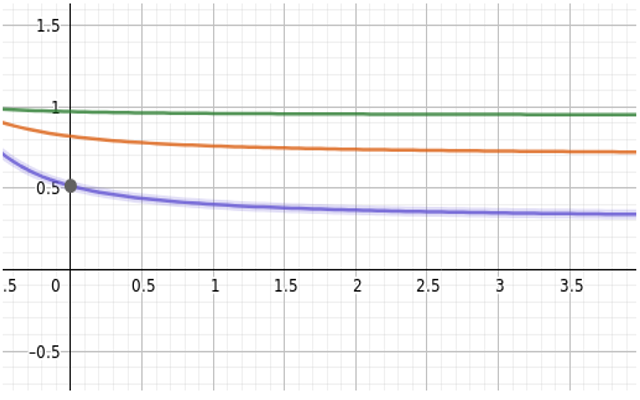
\includegraphics[scale=0.5]{./images/fitness.png}
\caption{Evalution de forme d'entrainement pour plusieurs valeurs de y}
\label{fonction}
\end{figure}

\vspace{0.8cm}

\begin{multicols}{2}
Au début, nous créons une population de plusieurs réseaux de neurones que nous formons séparément à partir de différents paramètres de départ (structure, poids et biais). Lors de l'analyse, nous pouvons utiliser le calcul de tous ces réseaux. Comme ils ont commencé leur formation à partir de différentes configurations, ils n’ont probablement pas convergé vers le même minimum de fonctions, nous avons donc augmenté la probabilité de nous approcher d’un minimum global.
\\
Nous utilisons toutes les suppositions de tous les réseaux de la population pour obtenir le temps que nous essayons de prévoir. Ensuite, après l’interruption de l’application, nous appliquons la fonction de mise en forme introduite ci-dessus pour évaluer individuellement les réseaux (Figure ~\ref{pop}) et nous générons la prochaine génération à l’aide des réseaux les plus performants. Pour effectuer la sélection, nous normalisons tout le score de sorte que la somme totale soit de $1$ et nous sélectionnons certains réseaux au hasard. Plus leur score est élevé, plus la probabilité d'être sélectionné est grande.
\end{multicols}

\vspace{0.8cm}

\begin{figure}[!ht]
\centering
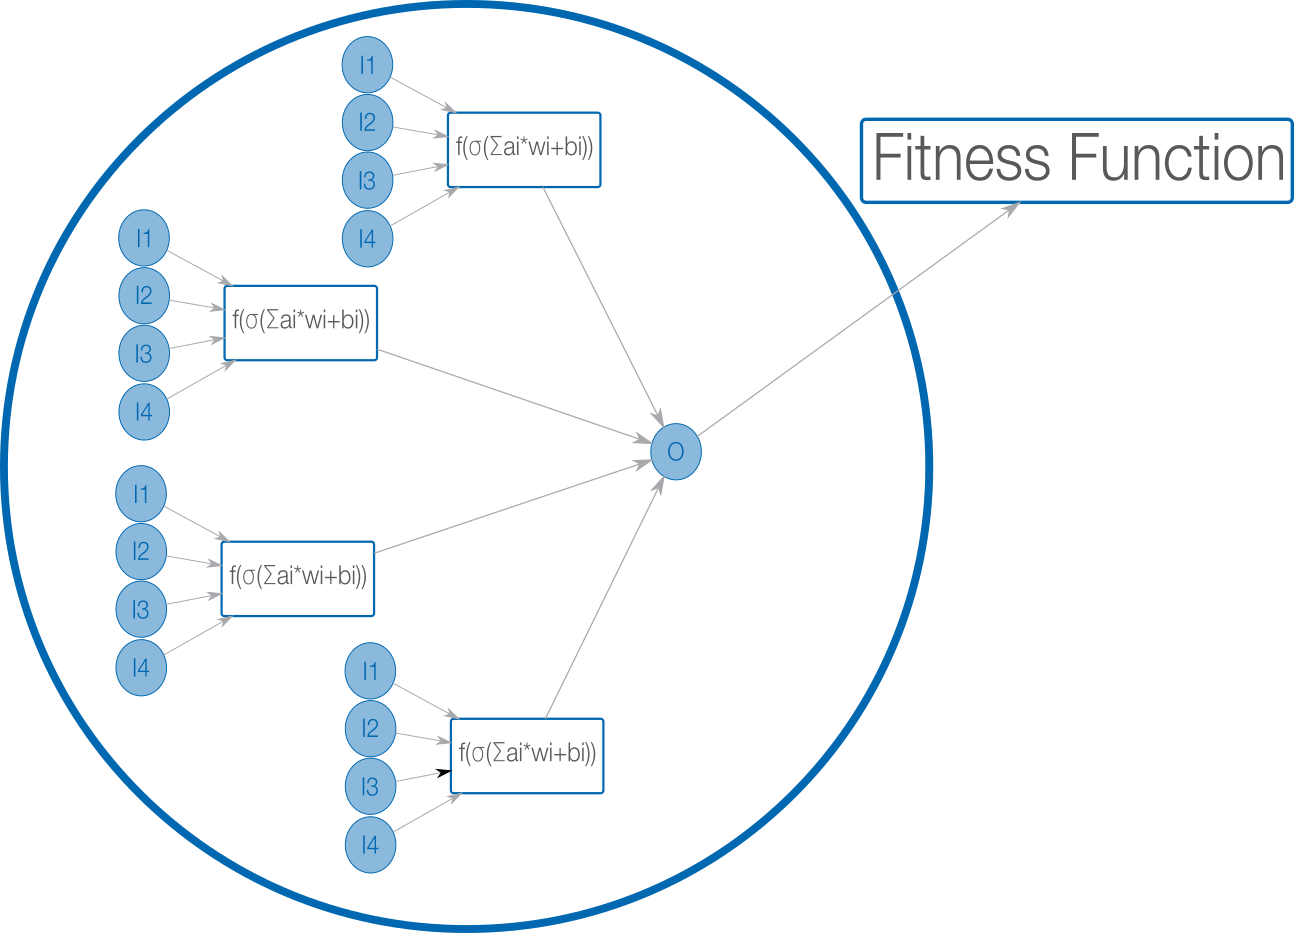
\includegraphics[scale=0.5]{./images/PNG/Population.png}
\caption{Une population de reseau}
\label{pop}
\end{figure}

\vspace{0.8cm}

\begin{multicols}{2}
Au cours du processus, nous ajoutons également de petites mutations aux hyperparamètres afin d’avoir moins de chances de rester bloqués dans une configuration non optimale. Cette méthode a également résolu le problème du choix de l’ensemble des hyperparamètres, car ils évoluent tout au long de l’exécution de l’algortihm.
Avec deux réseaux donnés, un autre est créé en générant une liste vide que nous remplissons avec des éléments d'une liste ou l'autre avec une probabilité $\frac{1}{2}$. Puis, avec une petite probabilité appelée $mutation ~rate$, nous introduisons des mutations qui peuvent être soit une petite variation d’un nombre entier dans les listes, soit la taille de chaque liste.


\subsection{Conclusions et limitations}
Cette méthode peut être assez efficace car nous pouvons également collecter des données d’exercices antérieurs pour déterminer la meilleure structure pour commencer le principe génétique, ce qui pourrait être perçu comme une autre forme d’apprentissage. Cependant, même si une partie de celle-ci pourrait être utile, la méthode complète n'est pas réalisable car elle n'est pas adaptée aux nouvelles architectures d'applications standard. En effet, l'ensemble du processus repose sur la formation de réseaux de neurones réalisée à l'aide d'une architecture spécifique de l'application et ne doit pas évoluer pendant l'exécution de l'algorithme pour deux raisons majeures. La première est que l'apprentissage serait, dans le meilleur des cas, beaucoup moins efficace et le second problème est que la comparaison est faite coordonnée par coordonnée avec une image calculée à partir de données historiques. Ainsi, nous ne pouvons pas comparer les nouvelles images avec l'ancienne moyenne et tout l'algorithme s'effondre.

Cela suggère un chemin possible. Nous devrions trouver un moyen d'identifier les variables de l'application qui ont le plus d'impact. C'est une question intéressante car identifier ces variables permettrait non seulement de limiter le nombre de données utilisées pour alimenter le réseau de neurones, mais permettrait également d'en ajouter de nouvelles sans interrompre directement l'entraînement. En effet, si la variable nouvellement introduite est importante, la formation pourrait être effectuée ultérieurement sans empêcher la comparaison. De plus, il s'agirait d'une information pertinente pour faciliter le diagnostic d'une application. C'est pourquoi la partie suivante portera sur l'identification de ces variables. Dans cet esprit, l'analyse des données brutes sera plus pertinente et nous n'utiliserons donc pas les données d'état de surveillance, mais directement les valeurs obtenues à partir de capteurs. Par conséquent, une nouvelle méthode d'apprentissage sera éventuellement explorée.


\section{Améliorations des données brutes}
Nous avons besoin de plus d’adaptabilité car les applications existantes ne modifiaient pas souvent leur architecture, elles ont été conçues selon le schéma figure~\ref{omodl}. Ce modèle n’a cependant pas permis beaucoup d’optimisations. Par conséquent, maintenant, pour s’adapter à la demande, les applications sont maintenant basées sur un modèle plus horizontal ou distribué, comme illustré à la figure~\ref{nmodl}. Cela entraîne une modification plus fréquente des infrastructures de l'application. Ce problème sera discuté dans la partie suivante.

\end{multicols}

\begin{figure}[!ht]
\centering
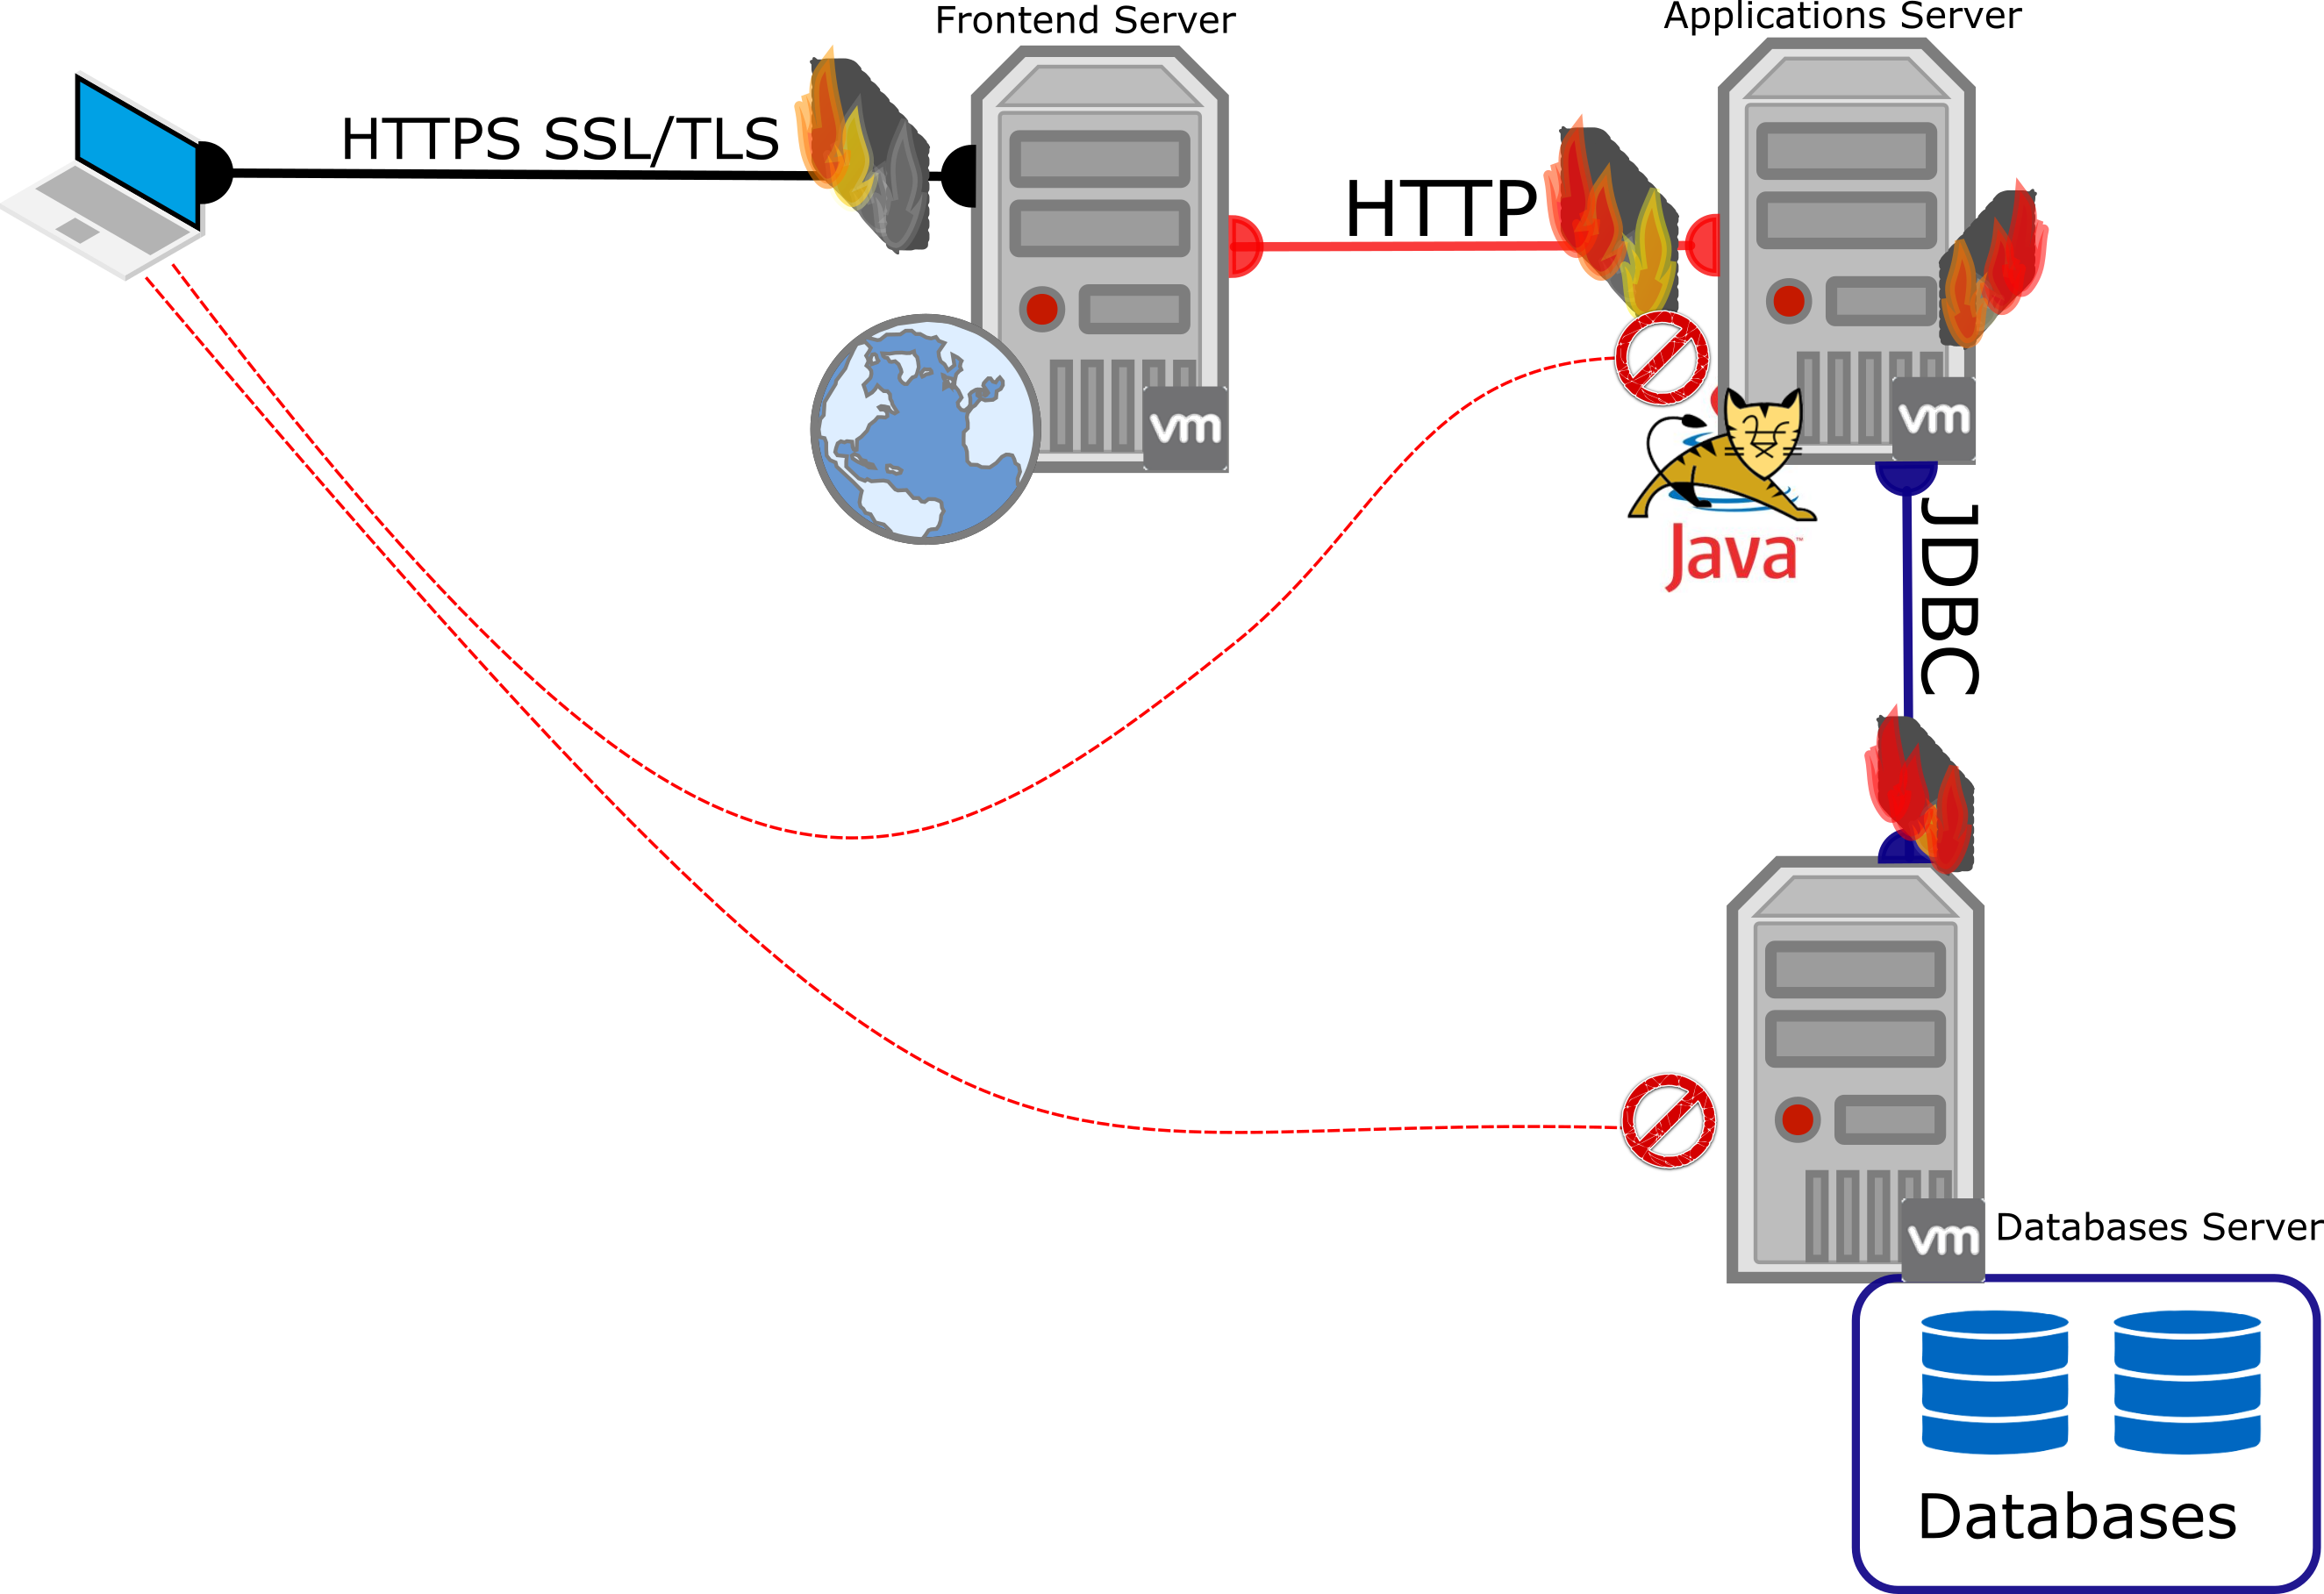
\includegraphics[scale=0.40]{./images/PNG/Application_legacy.png}
\caption{Architecture dite Legacy}
\label{omodl}
\end{figure}

\vspace{0.5cm}

\begin{figure}[!ht]
\centering
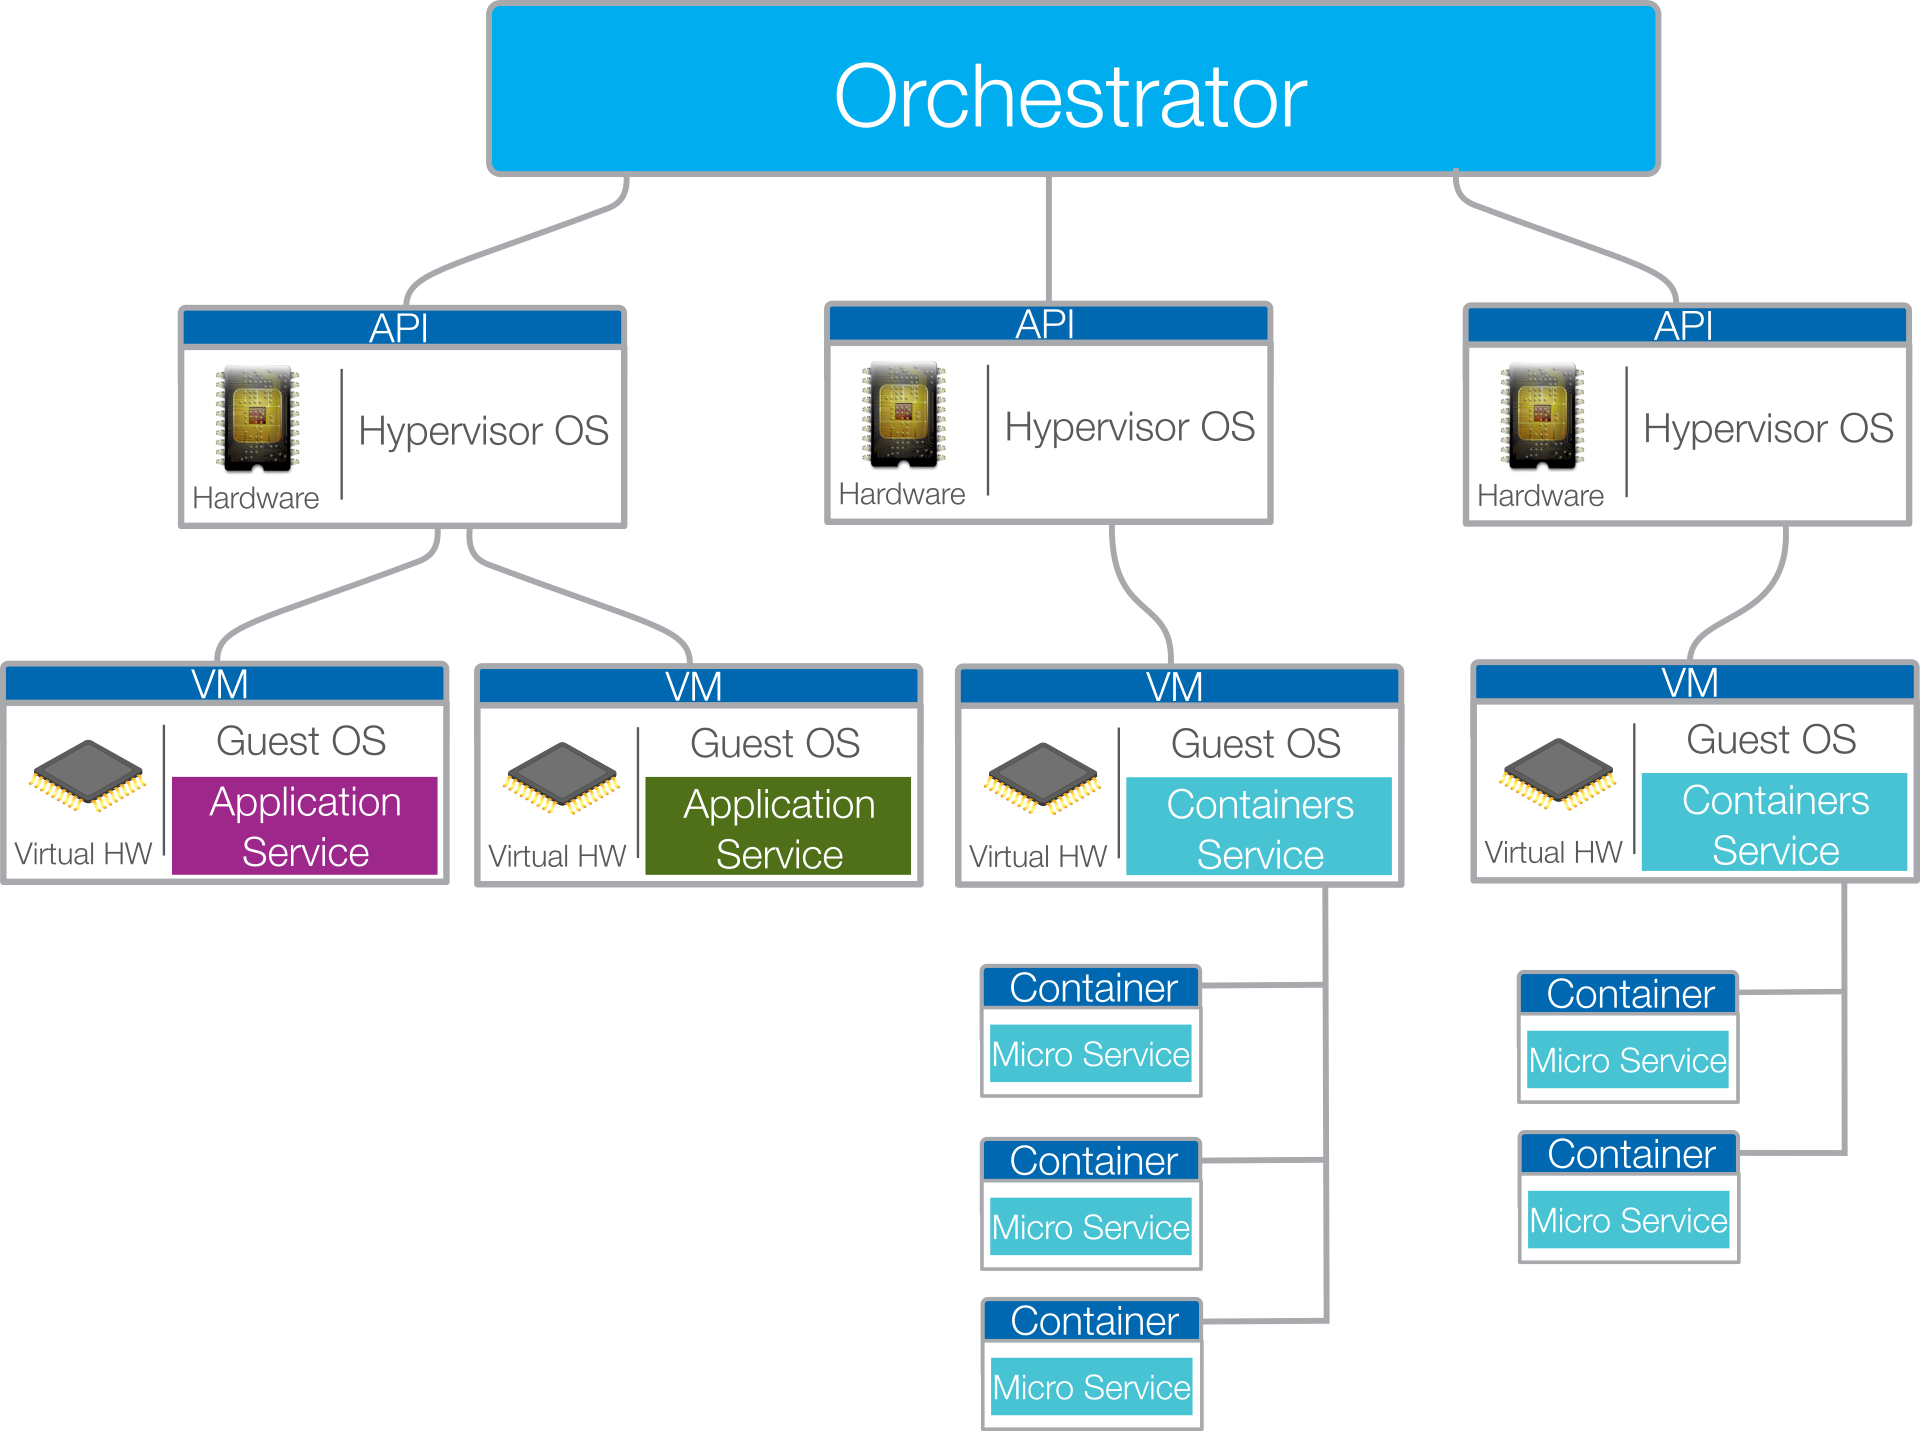
\includegraphics[scale=0.60]{./images/PNG/micro_archi.png}
\caption{Architectures en nuages et microservices}
\label{nmodl}
\end{figure}


\begin{multicols}{2}
Nous étendons ici notre champ de possibilité à tous les types de données car nous devons résoudre le problème de rigidité de la méthode précédente. Nous allons d’abord essayer de trouver un moyen de sélectionner les hôtes les plus influents de l’application, c’est-à-dire les hôtes pour lesquels une variation de comportement a un impact important sur l’ensemble de l’application. Ensuite, nous trouverons un moyen d'organiser les hôtes en groupes ayant des comportements communs afin d'analyser la moyenne du groupe total. Une fois cela fait, nous pourrons ajouter et supprimer des hôtes de ces groupes sans perdre l'apprentissage. Nous nous attendons à ce qu’il permette également d’utiliser davantage de données lors de la formation de l’algorithme.
\end{multicols}

\vspace{0.8cm}

\begin{multicols}{2}

\subsection{Selection par fonctions}
\subsubsection{Gestion du signal}
Le signal que nous recevons des données historiques est plein de petites variations qui peuvent être dues à des erreurs de mesure ou à des changements de parasite périodique qu’il est inutile de traiter. Nous allons donc essayer d’éliminer le plus de bruit possible afin d’obtenir une meilleure précision dans le calcul de l’influence. En effet, nous allons utiliser une corrélation entre les signaux pour deviner l’influence d’une variable sur une autre, nous ne devons donc prendre en compte que l’événement significatif. De plus, nous devons trouver un moyen approprié d’évaluer l’influence d’un nœud sur un autre. Cet aperçu de notre approche est décrit à la figure~\ref{trng}.
\end{multicols}

\vspace{0.8cm}

\begin{figure}[!ht]
\centering
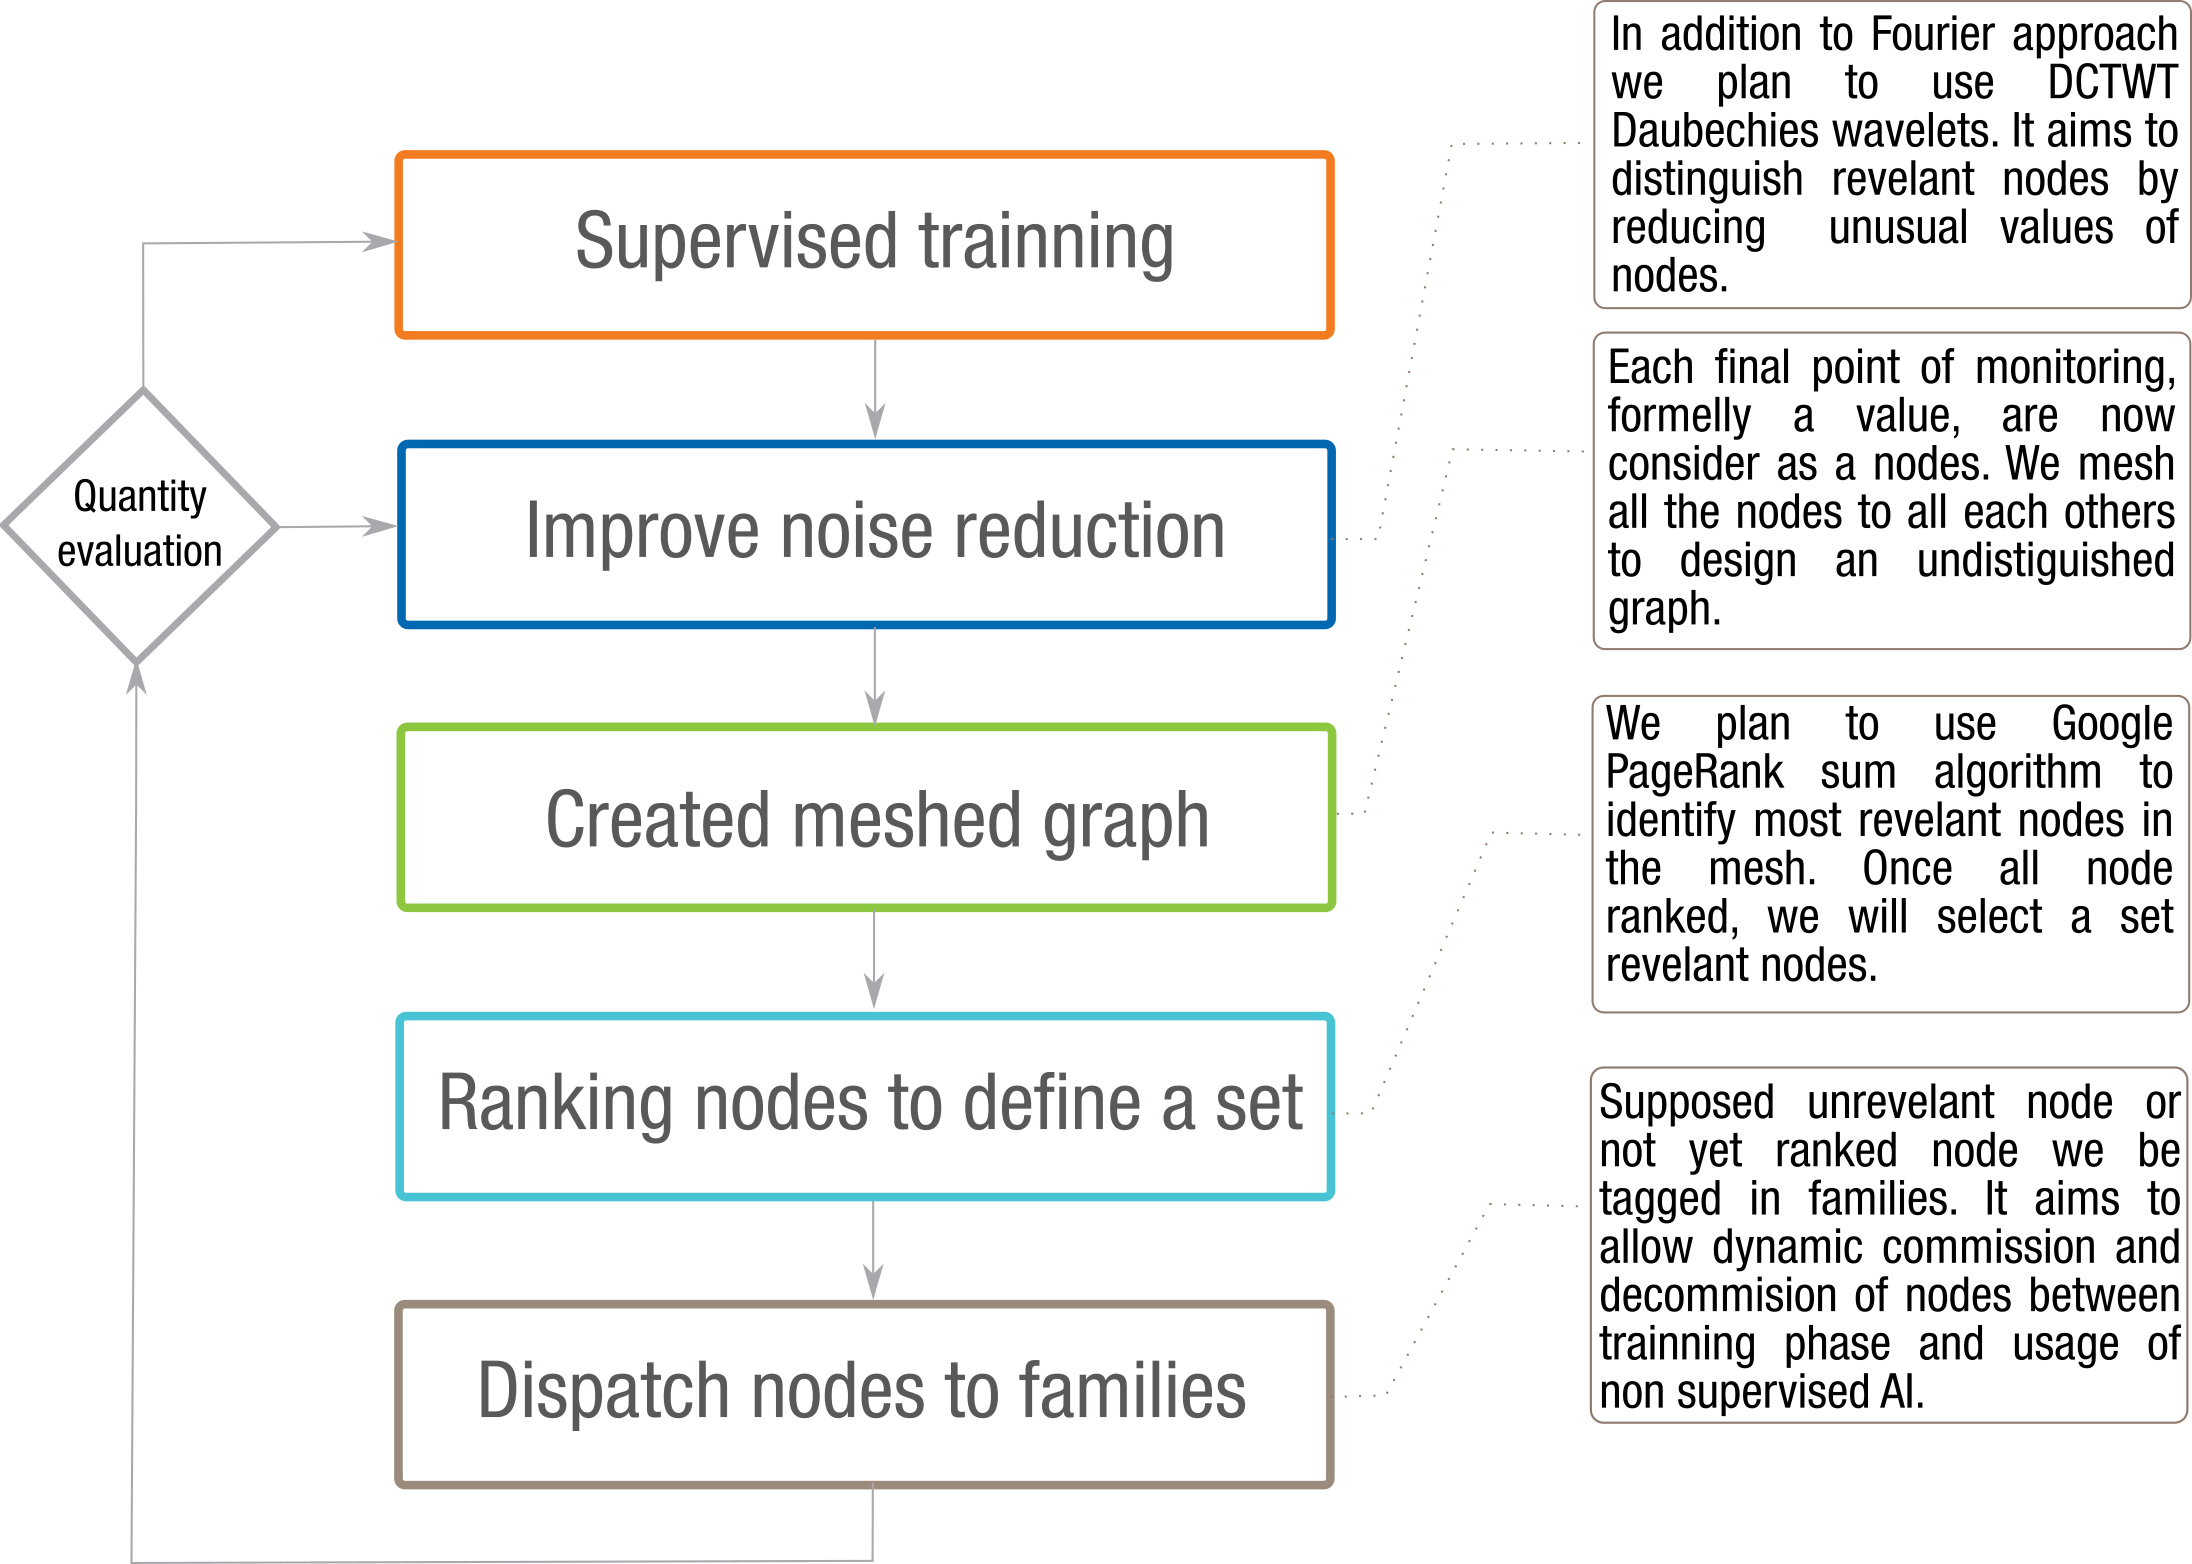
\includegraphics[scale=0.8]{./images/Apprentissage_V2.png}
\caption{Phase d'entrainement}
\label{trng}
\end{figure}

\vspace{0.8cm}

\begin{multicols}{2}
Afin de réduire le bruit dans notre signal, nous allons utiliser une théorie des ondelettes. La méthode choisie est décrite en détail dans ~\cite{ref1}. Fondamentalement, nous transformons les données en wavelet domain avec DTCWT - ce qui peut être fait avec la bibliothèque dtcwt en python par exemple (voir le code dans la documentation ci-dessous) - nous effectuons ensuite le traitement, il consiste à réduire le coefficient de bruit et finalement nous récupérons le signal débruit en faisant la transformation inverse.
\end{multicols}
\begin{lstlisting}[language=Python, caption=Exemple d'utilisation de la librairie DTCWT avec Python]
from matplotlib.pylab import *
import dtcwt


# 1D transform, 5 levels
transform = dtcwt.Transform1d()
vecs_t = transform.forward(vecs, nlevels=5)

# Inverse
vecs_recon = transform.inverse(vecs_t)
\end{lstlisting}


\begin{multicols}{2}
La transformation est une décomposition de la fonction en une somme d'un coefficient multiplié par chaque vecteur d'une famille d'ondelettes ayant des propriétés spécifiques (la théorie est expliquée en détail dans l'article). dans ce travail, nous utiliserons les ondelettes de Daubechies (db11 Figure~\ref{db}}) qui ont été choisies avec ~\cite{ref2} et des documents référencés.
\end{multicols}

\begin{figure}[!h]
\centering
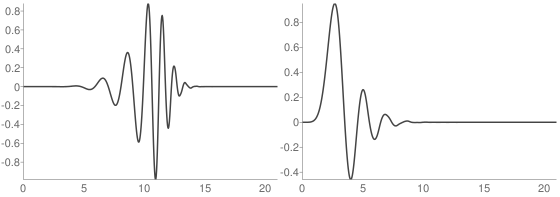
\includegraphics[scale=0.67]{./images/PNG/db11.png}
\caption{Fonction de mise à l'échelle et d'ondelettes}
\label{db}
\end{figure}

\begin{multicols}{2}
\subsubsection{Influence evaluation}
Dans cette partie, il est nécessaire de rappeler que ce que nous faisons est fait avant l'exécution de l'application pendant une phase d'apprentissage. Par conséquent, nous n’avons aucune contrainte temporelle et l’algorithme peut être lent.
\\
Notre objectif est de mettre en œuvre un moyen d'évaluer l'influence de chaque hôte et service l'un sur l'autre. Nous pouvons visualiser cette idée sous forme de graphique où les nœuds sont les hôtes et les services et les contours sont orientés. L'arête $(s_i,s_j)$ est liée à la valeur de l'influence que $s_j$ a sur $s_i$, voir la figure ~\ref{graphe}.
\end{multicols}


\begin{figure}[!h]
\centering
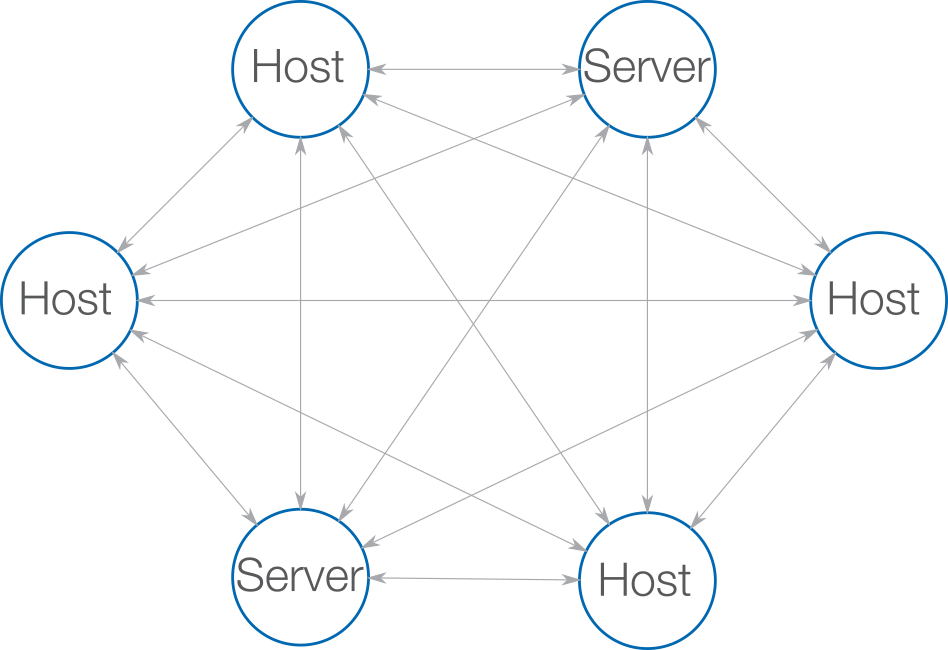
\includegraphics[scale=0.6]{./images/PNG/Graphe.png}
\caption{Exemple de graph}
\label{graphe}
\end{figure}

\begin{multicols}{2}
L’influence est supposée être dans notre cas le flux d’information entre $s_i$ et $s_j$, donc en utilisant le flux d’information de Liang-Kleeman ~\cite{ref3} sur certaines données dont nous disposons, nous pouvons calculer la valeur des arêtes du graphique.

\subsubsection{Ciblage des équipements influent}
Nous voulons maintenant trier les nœuds en fonction de l’influence qu’ils exercent sur le graphe. Nous allons utiliser le principe de l'algorithme de $page~rank$ ~\cite{ref4} sur le graphe où la probabilité de suivre une arête est donnée par valeur d'influence. Cela est toutefois légèrement différent de l'algorithme PageRank classique car les arêtes ont des poids. Intuitivement, cela peut être vu comme une marche aléatoire dans le graphique avec la probabilité de suivre un bord proportionnel à son poids.

Cependant, pour le calculer, nous utiliserons la méthode dite Power, qui est un moyen simple et rapide de le calculer. En laissant $M$ la matrice de transition entre les nœuds, on l'obtient en normalisant les scores des arêtes sortant d'un nœud et en les utilisant comme probabilité. Nous calculons le vecteur de rang $X$ en commençant par un $X_0$ arbitraire, puis en utilisant:

	\[X_{t+1} = (dM + \frac{1-d}{N}J_N)X_t\]
Jusqu'à atteindre :
	\[ \mid{X_t+1 - X_t}\mid < \epsilon\]
ou $\epsilon$ est un paramètre relativement petit, $N$ est le nombre total de nœuds dans le graphe, c’est-à-dire le nombre d’hôtes et de services dans l’application, $J_N$ est la matrice carrée de taille N contenant uniquement des uns et enfin $d$ est un paramètre qui représente la probabilité d’arrêter la marche aléatoire fixée à $0.85$, car l’expérimentation de Google a montré que c’est la valeur optimale pour avoir un taux convergent décent et une chance d’atteindre le vecteur $X$ que nous calculons.
\end{multicols}

\begin{lstlisting}[language=Python, caption=Methode Power en Python]
import numpy as np

def pagerank(M, eps, d=0.85):
    N = M.shape[1]
    X = np.random.rand(N, 1)
    X = X / np.linalg.norm(X, 1)
    X_{t-1} = np.ones((N, 1), dtype=np.float32) * np.inf
    T = (d * M) + (((1 - d) / N) * np.ones((N, N), dtype=np.float32))
    
    while np.linalg.norm(X - X_{t-1}, 2) > eps: 
        X_{t-1} = X
        X = np.matmul(T, X)
    return X

\end{lstlisting}

\begin{figure}[!h]
\centering
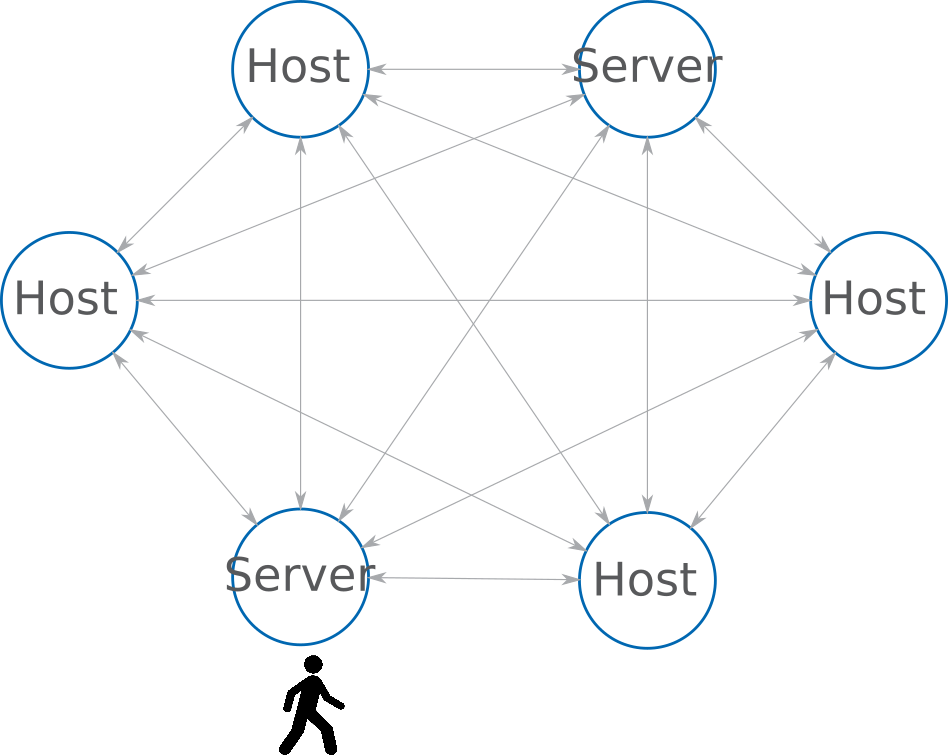
\includegraphics[scale=0.5]{./images/PNG/GraphesRandomWalk.png}
\caption{Parcours aléatoire: Etat initiale}
\label{graphrwb}
\end{figure}

\begin{figure}[!h]
\centering
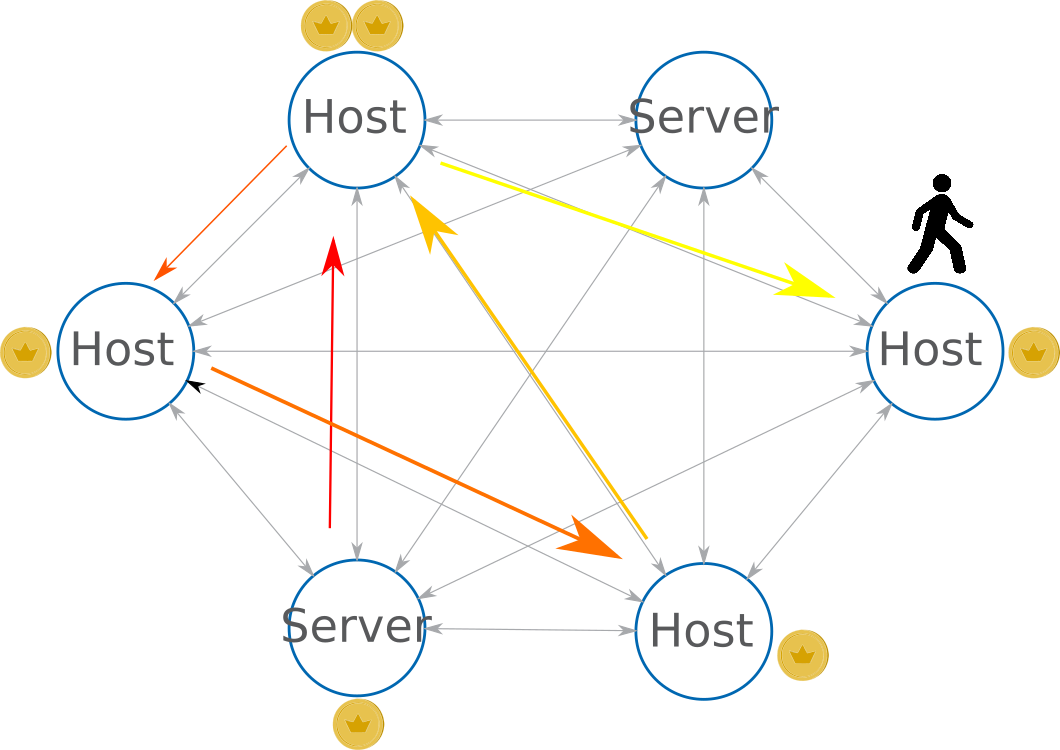
\includegraphics[scale=0.5]{./images/PNG/GraphesRandomWalk2.png}
\caption{Parcours aléatoire: Etat avancé}
\label{graphrw}
\end{figure}

\begin{multicols}{2}
\subsubsection{Conclusions}
En utilisant ces différentes techniques, nous parvenons à obtenir un sous-ensemble de tous les hôtes et services qui sont ceux qui ont le plus d’influence sur l’ensemble de l’application. Nous pouvons concentrer notre apprentissage sur ces variables particulières. Ce qui signifie que nous aurons moins souvent à gérer les modifications architecturales de l'application. Cela devrait également alléger les calculs lors de la phase d'apprentissage. Cependant, nous allons essayer d'obtenir plus d'informations en regroupant les autres variables afin d'assurer la flexibilité de l'application et des calculs légers.\\
\subsection{Groupement de fonctionnalitées}
Enfin, lorsque nous avons sélectionné nos principales fonctionnalités, nous avons regroupé toutes les autres afin de pouvoir nous adapter aux modifications de l’architecture de l’application. Nous avons supposé que les variables qui seront supprimées et ajoutées le plus souvent ont également un impact limité sur l'application globale.\\
Nous allons utiliser la mise en cluster du processus de voisinage la plus proche décrite dans cet article ~\cite{ref5} (qui expose également un algorithme de moyenne K mais celui-ci est dit moins efficace avec une petite quantité de données, ce qui peut être le cas dans notre cas.) et nous utiliserons ensuite la méthode décrite dans la première partie sur les fonctionnalités sélectionnées et une moyenne de celles de chaque cluster.
\end{multicols}

\vspace{0.8cm}

\bibliography{biblio}{}
\bibliographystyle{plain}


\end{document}

